\slide{Conclusão}{
    \begin{itemize}
        \item TODO
    \end{itemize}
}

\slide{Trabalhos Futuros}{
    \begin{itemize}
        \item Treinar os modelos com pelo 1 ano de dados;
        \item Polir a representação da coluna Data para os modelos;
        \item Aplicar os modelos desenvolvidos a um conjunto de dados referente a vias livres;
        \item Utilizar múltiplos sensores para predição;
        \item Utilizar modelos paramétricos;
        \item Incluir modelos não paramétricos mais complexos;
        \item Aprofundar a escolha de hiper-parâmetros;
        \item Incluir modelos diferentes;
    \end{itemize}
}

\slide{Dados e Código}{
    \begin{itemize}
        \item Código utilizado se encontra em:  \url{https://github.com/claudiosegala/Monografia/tree/master/code}
        \item Dados utilizados se encontram em: \url{http://bit.ly/processed-data-2l5MaAG}
    \end{itemize}
}

% \slide{Códigos}{
%     \begin{figure}[]
%         \centering
%         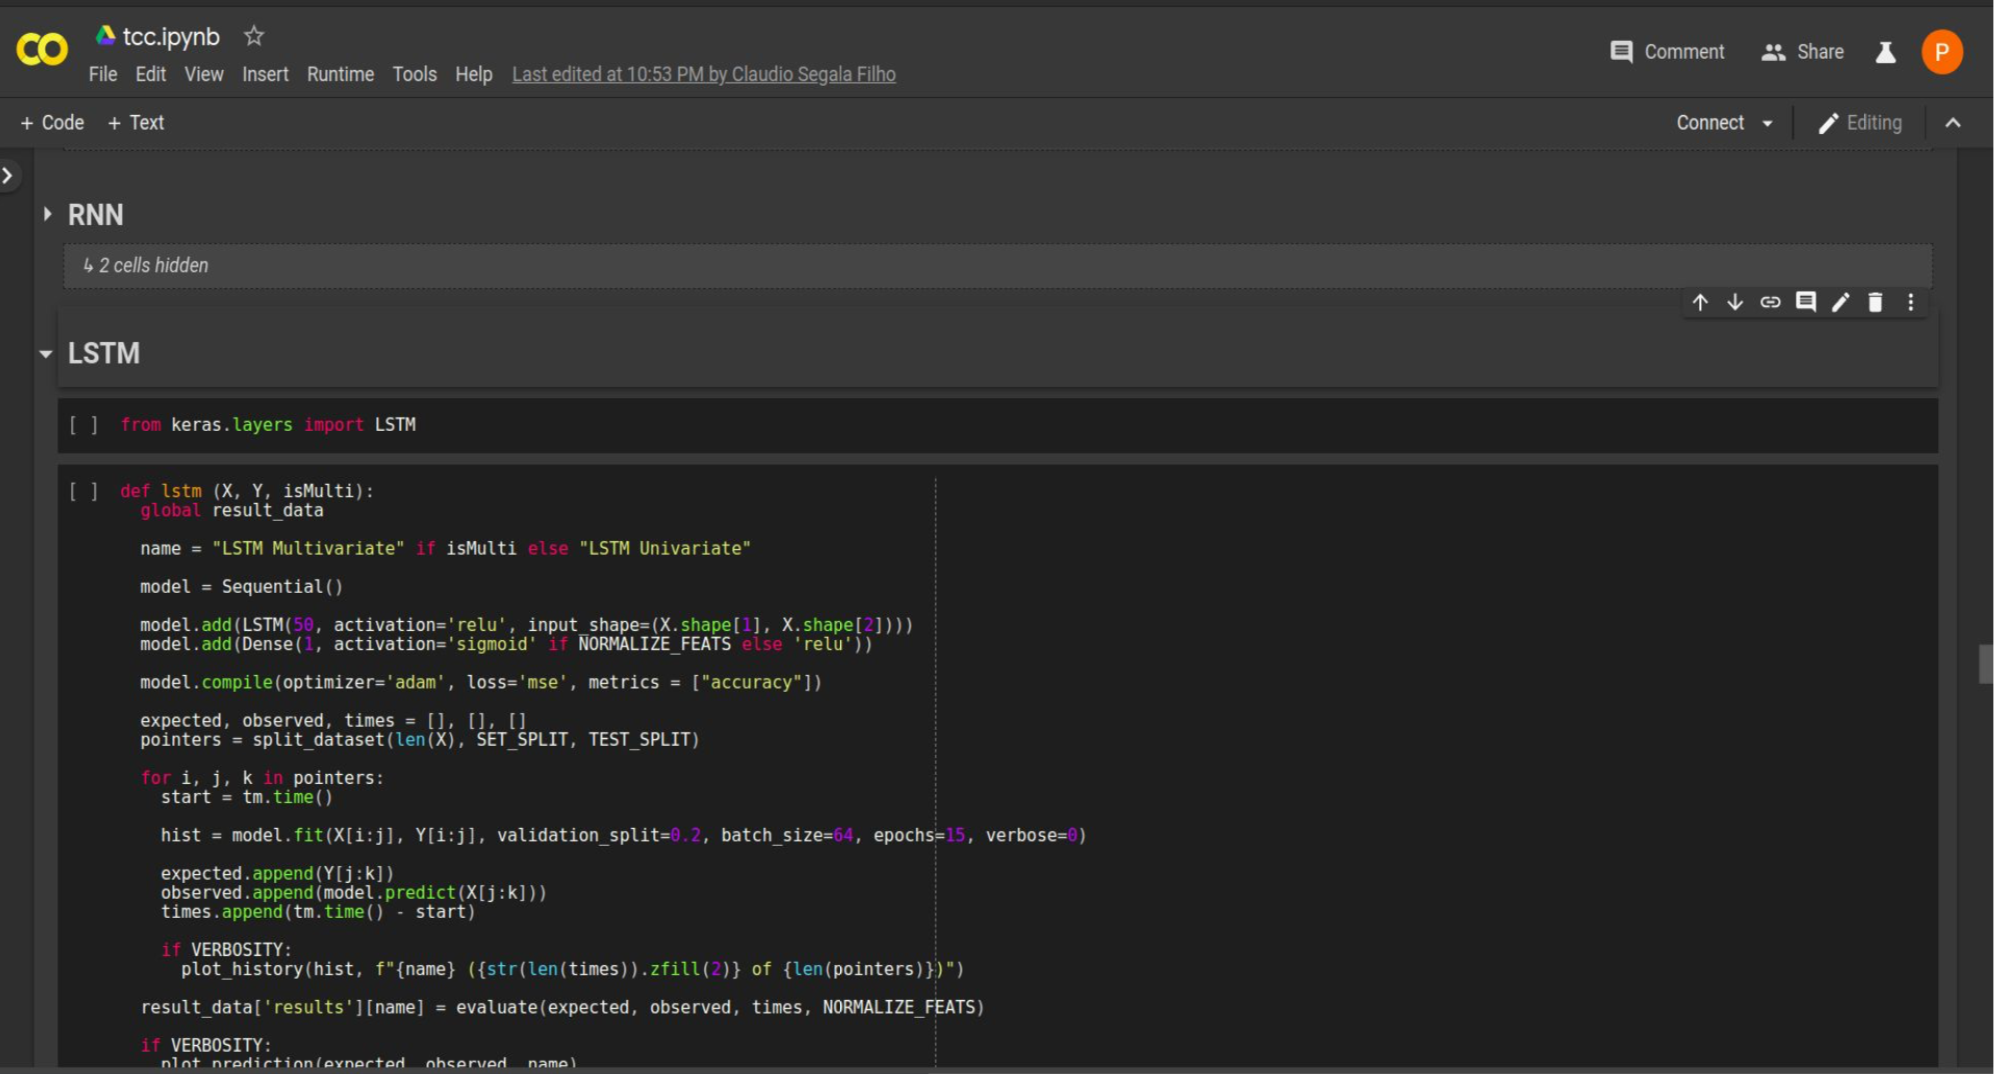
\includegraphics[scale=0.25]{img/colab.png}
%         \caption{Código utilizado disponível na plataforma Google Colab}
%         \label{fig:colab}
%     \end{figure}
% }

% \slide{Dados}{
%     \begin{figure}[]
%         \centering
%         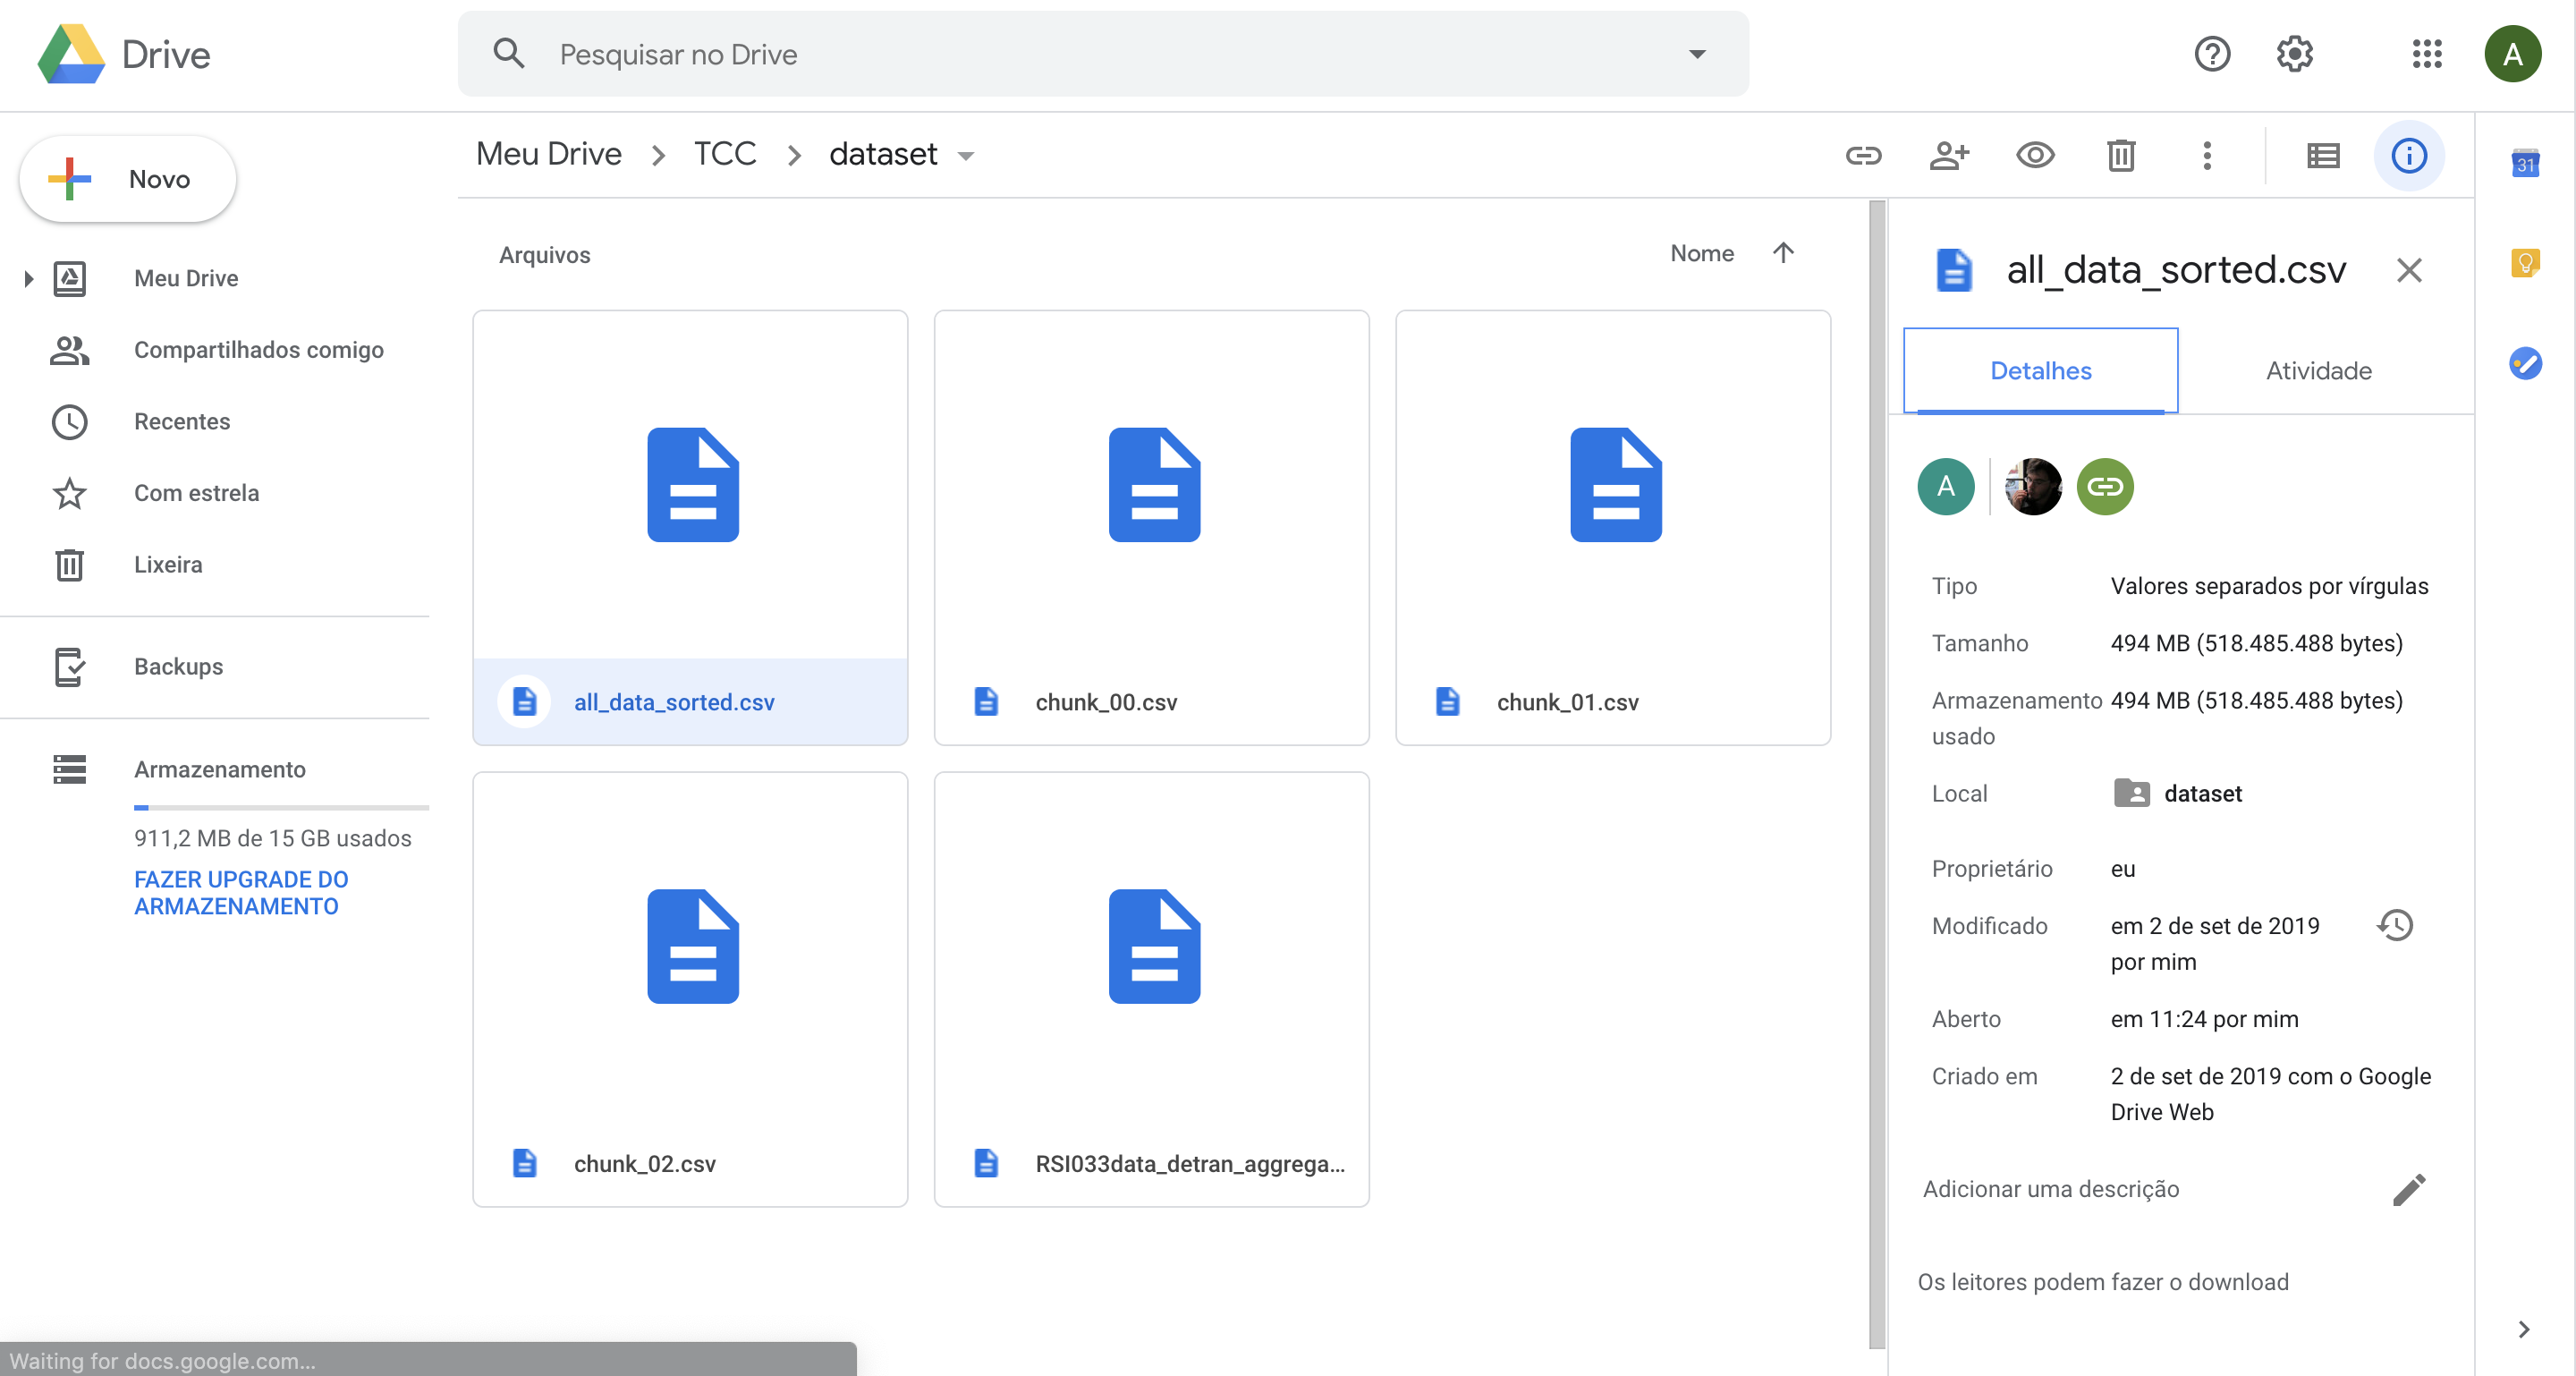
\includegraphics[scale=0.25]{img/dataset_drive.png}
%         \caption{Dados utilizado disponível na plataforma Google Drive}
%         \label{fig:dataset_drive}
%     \end{figure}
% }